%---------------------导言区---------------------------%
\documentclass[12pt,a4paper,UTF8]{ctexart}
\usepackage{geometry}
	\geometry{left=2.5cm,right=2.5cm,top=3.2cm,bottom=2.8cm}
\usepackage{xeCJK,amsmath,paralist,enumitem,booktabs,multirow,graphicx,subfig,setspace,listings,lastpage}
	\setlength{\parindent}{2em}
	\lstset{language=Python}
\usepackage{fancyhdr}
	\pagestyle{fancy}
	\rhead{B12 温度测控仪的设计和组装}
	\lhead{基础物理实验\uppercase\expandafter{\romannumeral2}简要实验报告}
	\cfoot{Page \thepage/\pageref{LastPage}}  %当前页\总页数
	\rfoot{\today}
	\renewcommand{\headrulewidth}{0.4pt}
	\renewcommand{\theenumi}{(\arabic{enumi})}
\usepackage[colorlinks,linkcolor=blue,urlcolor=blue,citecolor=blue]{hyperref}
%%%%%%%%%%%%%%%%%%%%%%%%%%%%%%%%%%%%%%%%%%%%%%%%%%%%%%%%%%
%%%%%%%%%%%%%%%%%%%%%%%%%正文开始%%%%%%%%%%%%%%%%%%%%%%%%%%
%%%%%%%%%%%%%%%%%%%%%%%%%%%%%%%%%%%%%%%%%%%%%%%%%%%%%%%%%%

\begin{document}

%%begin-------------------标题与信息-----------------------%%
%%标题
\begin{center}
\LARGE\textbf{B12 温度测控仪的设计和组装}
\end{center}

%%信息
\begin{doublespacing}
	\centering
	\begin{tabular}{ll}
	 & \\
	{\CJKfontspec{Droid Sans Fallback} 实验人:黄子维 20980066} & {\CJKfontspec{Droid Sans Fallback}合作者:黄睿杰 20980062}\\
	{\CJKfontspec{Droid Sans Fallback} 实验时间:2021.12.5~星期四~上午} & {\CJKfontspec{Droid Sans Fallback} 室温:21$^{\circ}$C~相对湿度:45\%}
	\end{tabular}
\end{doublespacing}
%%end-------------------标题与信息-----------------------%%

\subsection*{【数据处理及分析】}
	\subsubsection*{1. 温度测控仪的组装和测试}
		\paragraph{组装温度测控仪电路}~
        \newline
		\indent
        温度测控仪电路如图\ref{fig:illus-1}所示。最终组装电路如图\ref{fig:illus-2}。
		\begin{figure}[htbp]
			\centering
			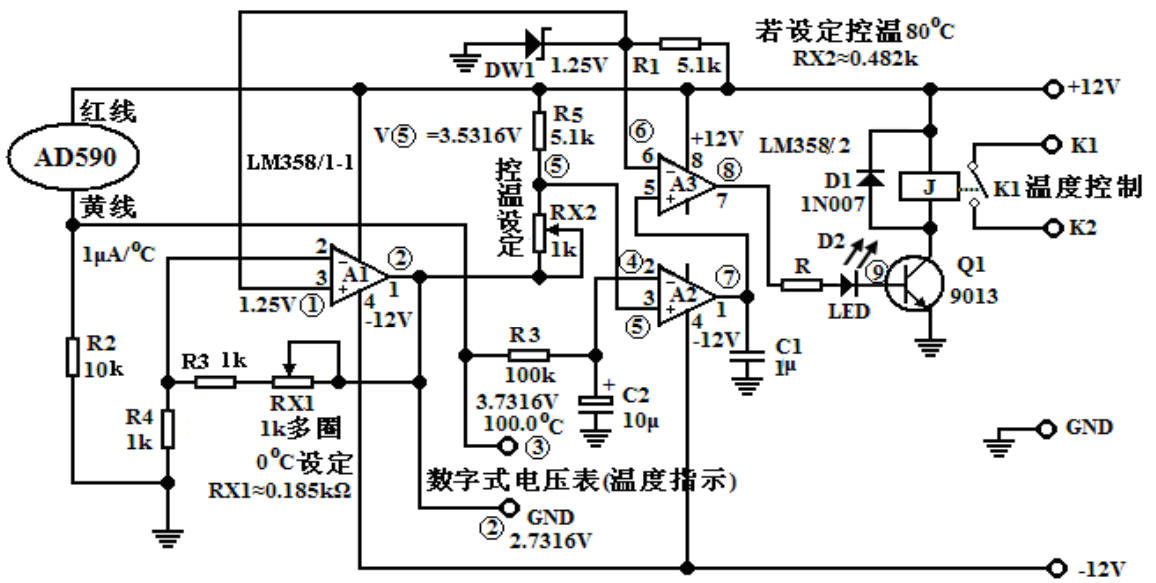
\includegraphics[width=0.7\textwidth]{attachments/illus-1.png}
			\caption{温度测控仪电路图}
			\label{fig:illus-1}
		\end{figure}
		\begin{figure}[htbp]
			\centering
			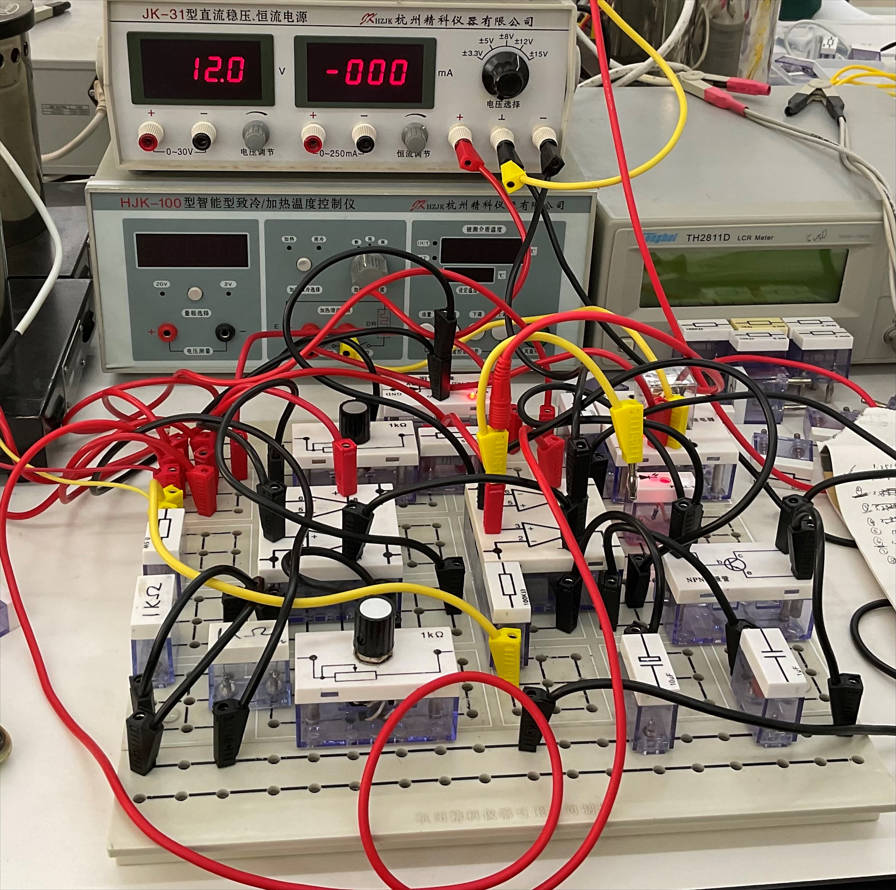
\includegraphics[width=0.4\textwidth]{attachments/illus-2.jpg}
			\caption{温度测控仪组装示意图}
			\label{fig:illus-2}
		\end{figure}
        \paragraph{检查电路测试点}~
        \newline
		\indent
        适当调节可变电阻$RX1$和$RX2$,根据电路图标注,使用万用表检查测试点电压,结果如表\ref{tab:1}所示。
        \begin{table}[htbp]
            \centering
                \begin{tabular}{cc}
                    \toprule
                    测试点	&电压$/V$  \\
                    \midrule
                    $V_1$	&1.25154	\\
                    $V_2$	&2.73430	\\
                    $V_3$	&3.05109	\\
                    $V_4$	&2.86390	\\
                    $V_5$	&3.48478	\\
                    $V_6$	&1.39114	\\
                    $V_7$	&10.3144	\\
                    $V_8$	&9.3226 	\\
                    \bottomrule
                \end{tabular}
                \caption{\textbf{测试点电压}}
                \label{tab:1}
        \end{table}
        各测试点工作电压正常,继电器指示灯亮,电路正常工作。

    \subsubsection*{2. 使用温度测控仪控制加热阱恒温$75^oC$}
    依据$AD590$温度传感器测温原理
    \begin{equation}
        T = \frac{I}{K}
    \end{equation}
    其中温度系数$K_I \approx 1.0 \mu A/K$。若要控制加热阱温度恒温$75^oC$,则需调节可调电阻$RX2$使
    $V_5 \approx V_2 + 0.75 \approx 3.48430 V$。限于手动调整准确度,实验设置$V_5 = 3.48478 V$。
    打开加热阱,开始加热,观察设备工作状况。

    实验观察到温度测控仪继电器在温度达到$79.7^oC$时第一次断开,当温度下降至约$74^oC$时继电器再次闭合,
    此后温度逐渐趋近于稳定在$75^oC$附近,说明温度测控仪工作正常。
    温度测控仪继电器开闭对应温度如表\ref{tab:2}所示。实验记录见附图\ref{fig:2}。
    \begin{table}[htbp]
        \centering
            \begin{tabular}{ccc}
                \toprule
                继电器状态    &温度$/^oC$    &电压$/V$  \\
                \midrule
                $断开$   &79.7  &3.44765	\\
                $闭合$   &74.0  &3.44682	\\
                $断开$   &75.7	&3.44422	\\
                $闭合$   &73.8	&3.44355	\\
                $断开$   &75.4	&3.44320	\\
                $闭合$   &73.6	&3.44257	\\
                \bottomrule
            \end{tabular}
            \caption{\textbf{温度测控仪工作温度}}
            \label{tab:2}
    \end{table}
    \subsubsection{3. 标定AD590温度传感器}
    为更精确确定控温电压,我们对实验用AD590温度传感器进行了标定。标定结果如\ref{fig:1}
    \begin{figure}[htbp]
        \centering
        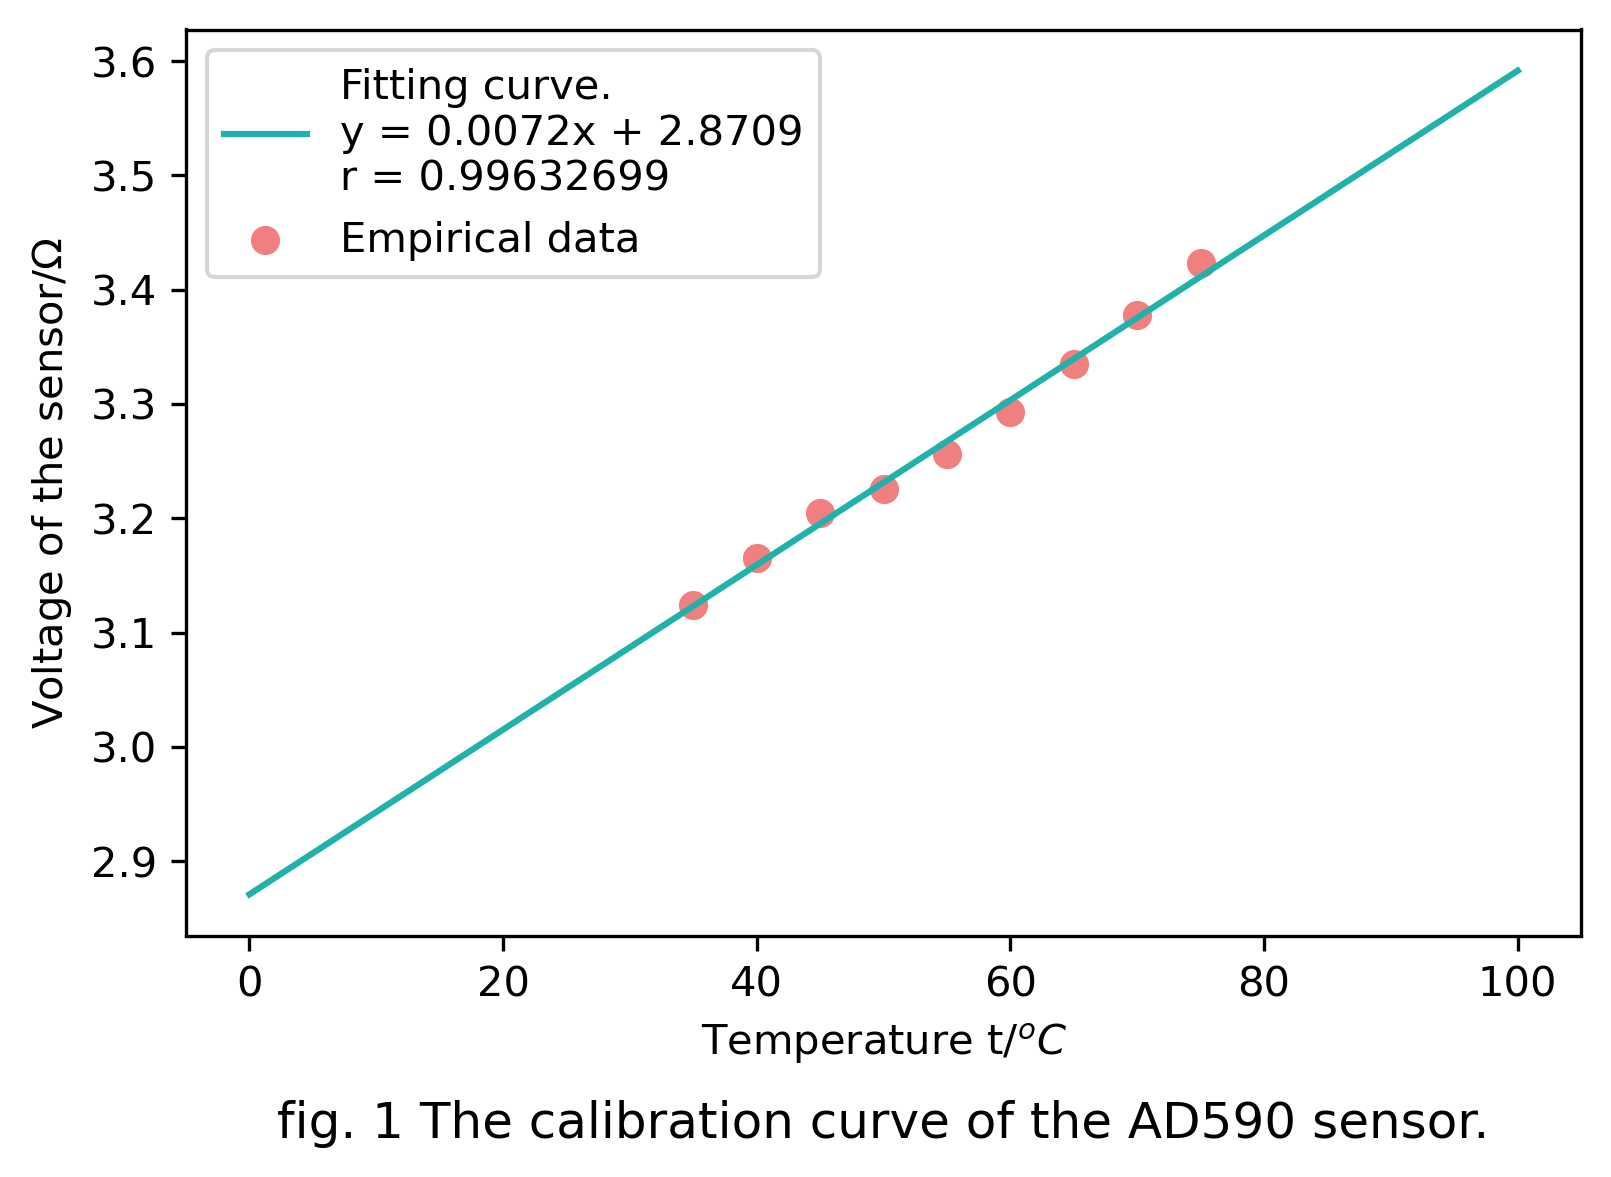
\includegraphics[width=0.4\textwidth]{attachments/fig.1.png}
        \caption{标定AD590}
        \label{fig:1}
    \end{figure}

    标定结果为温度系数$k_r = 7.2 mV/^oC$($R^2 = 0.996$),截距$U_0 = 2.8709 V$。
    标定结果与实验假设参数相差较大,然而温度传感器仍能正常工作。
    分析后我们认为,由于标定是在降温过程中进行的,所以可能存在较大误差。相关原因仍需进一步研究。

    \subsubsection{4. 其他两种温度测控仪工作原理}
    \paragraph{基于PT100/Cu50温度传感器的温度测控仪}~
    \newline
    \indent
    \begin{figure}[htbp]
        \centering
        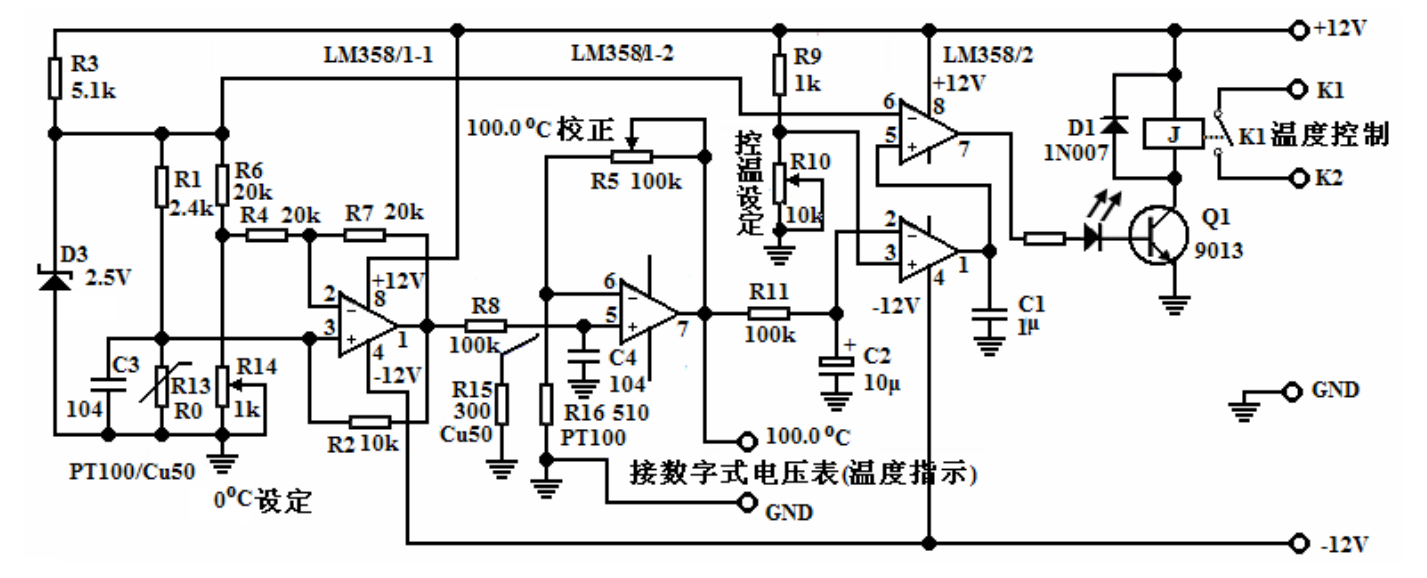
\includegraphics[width=0.4\textwidth]{attachments/illus-3.png}
        \caption{基于PT100/Cu50温度传感器的温度测控仪电路图}
        \label{fig:illus-3}
    \end{figure}
    温度显示:
    \begin{enumerate}[label=\arabic*.]
		\item 零度校准:将传感器置于零度环境,调节滑动变阻器$R14$使数字电压表取合适示数,设为$V_{0_1}$
		\item $100^oC$标定:记录温度传感器在$100^oC$下示数,设为$V_{0_2}$
		\item 依据电阻随温度线性变化关系$R_t = R_0(1+At)$,电压示数也应随温度线性变化。
        \item 依据电压温度系数$k = \frac{V_{0_2} - V_{0_1}}{100} V/^oC$可以计算任意电压示数$V$对应温度$T$($T = (V - V_{0_1})/k$)。
	\end{enumerate}
    温度控制:
    \begin{enumerate}[label=\arabic*.]
		\item 假设控温温度为$T_0$,则应调节滑动变阻器$R10$使测试点3电压为$V = V_{0_1} + kT_0$
		\item 当温度低于$T_0$时,$V_2 < V_3$,两个集成运放相继导通,LED点亮,继电器闭合,加热器开始工作。
        \item 当温度高于$T_0$时,$V_3 < V_2$,两个集成运放相继截止,LED点灭,继电器断开,加热器停止工作。
	\end{enumerate}

    \paragraph{基于LM35电压型温度传感器的温度测控仪}~
    \newline
    \indent
    \begin{figure}[htbp]
        \centering
        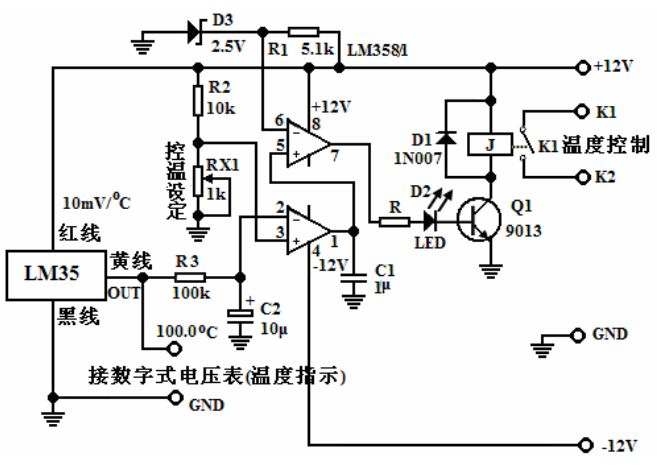
\includegraphics[width=0.4\textwidth]{attachments/illus-4.png}
        \caption{基于LM35电压型温度传感器的温度测控仪}
        \label{fig:illus-4}
    \end{figure}
    温度显示:
    \begin{enumerate}[label=\arabic*.]
        \item 温度$100^oC$时,输出电压$1.000V$,在温度变化范围$0 \sim 100^oC$内,电压随温度线性上升。
		\item 依据电压随温度线性变化关系$T = V/K_V ^oC$,其中电压温度系数$K_V = 10.0 mV/^oC$,即可根据电压示数求出温度。
	\end{enumerate}
    温度控制:
    \begin{enumerate}[label=\arabic*.]
		\item 假设控温温度为$T_0$,则应调节滑动变阻器$RX1$使测试点3电压为$V = K_VT_0$
		\item 当温度低于$T_0$时,$V_2 < V_3$,两个集成运放相继导通,LED点亮,继电器闭合,加热器开始工作。
        \item 当温度高于$T_0$时,$V_3 < V_2$,两个集成运放相继截止,LED点灭,继电器断开,加热器停止工作。
	\end{enumerate}
\subsection*{【思考题:列举其他若干种温度测控电路,分析原理】}
    \subsubsection*{1. 基于IC NE555的温度控制电路}
        电路核心元件为555时基集成电路,电路较为简单,控温效果好。电路图如\ref{fig:illus-5}
        \begin{figure}[htbp]
            \centering
            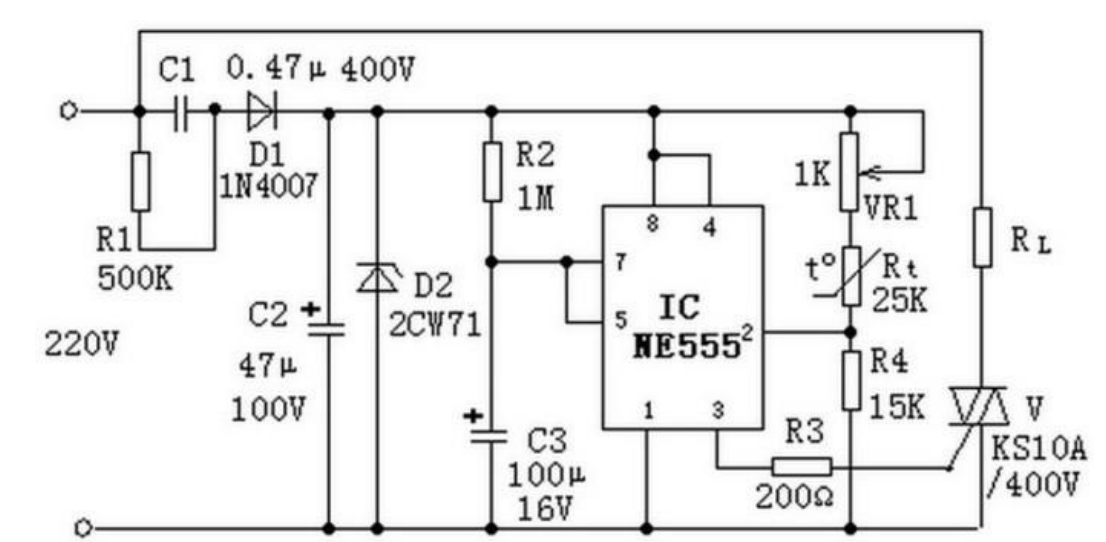
\includegraphics[width=0.4\textwidth]{attachments/illus-5.png}
            \caption{基于IC NE555的温度测控仪}
            \label{fig:illus-5}
        \end{figure}
        \paragraph{A. 元件选择} 
        电路控制元件为555时基集成电路(IC NE555),根据输入引脚电压大小比较输出高或低电平,控制加热器工作。
        热敏电阻$R_t$应选择合适阻值的负温度系数热敏电阻(如MF12或MF53)。
        滑动变阻器$VR1$阻值应合适,以获得较大调节范围以及保证设置灵敏度。
        \paragraph{A. 测温原理}
        \begin{enumerate}[label=\arabic*.]
            \item 假设控温温度为$T_0$,则应调节滑动变阻器$VR1$使$VR1 = 2R_4 - R_t(T_0)$
            \item 当温度低于$T_0$时,热敏电阻阻值大,引脚2为低电平,则引脚3输出高电平,双向晶闸管V导通,电加热器RL开始加热。
            \item 当温度高于$T_0$时,热敏电阻阻值小,引脚2为高电平,则引脚3输出低电平,双向晶闸管V断开,电加热器RL停止加热。
        \end{enumerate}
    \subsection*{2. 基于TW9205的冷断式温度控制电路}
    电路由TW9205及其外围元件组成的过零开关控制电路、可控硅驱动制冷控制电路及发声电路等组成。
    电路特点为“冷关断式”,常用于空调器、冰箱等制冷电路控温。电路图如\ref{fig:illus-5}
    \begin{figure}[htbp]
        \centering
        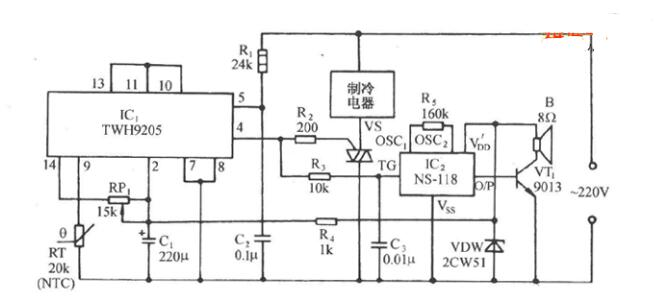
\includegraphics[width=0.4\textwidth]{attachments/illus-6.jpg}
        \caption{基于TW9205的冷断式温度控制电路}
        \label{fig:illus-6}
    \end{figure}
    \paragraph{A. 元件选择和连接} 
    温度传感器RT采用负温度系数(NTC)的热敏电阻,将它接在TWH9205芯片内的差动开关放大器的反相输入端(9脚)上;
    而差动开关放大器的正相输入端(13脚)与电位钳定端10、11脚相接,即13脚钳定在一个固定电位上。
    \paragraph{A. 测温原理}
    \begin{enumerate}[label=\arabic*.]
        \item 调节$RP1$电阻值,使在设定的温度以下TWH9205输出低电平,可控硅VS处于截止状态。
        \item 在温度升高到预定值后,热敏电阻$RT$阻值减小,TWH9205内差动开关放大器的输出状态发生变化,并在交流电源过零时TWH9205的输出端(4脚)转呈高电平,可控硅VS导通,制冷器运行。
        \item 环境温度下降,$RT$阻值升高,使集成电路内的差分开关放大器的反相输入端的电压也升高。当电压高于正相输入端的钳位电平时,在交流过零时又转呈低电平,可控硅VS截止,制冷器断电而停止运行。
        \item 如此循环往返,使被控设备或空间的温度保持在一定的温度范围内。
    \end{enumerate}

\subsection*{【附录:实验视频截图】}
继电器导通和断开瞬间截图如\ref{fig:2}
\begin{figure}[htbp]
    \centering
    \subfloat[第一次断开]{
    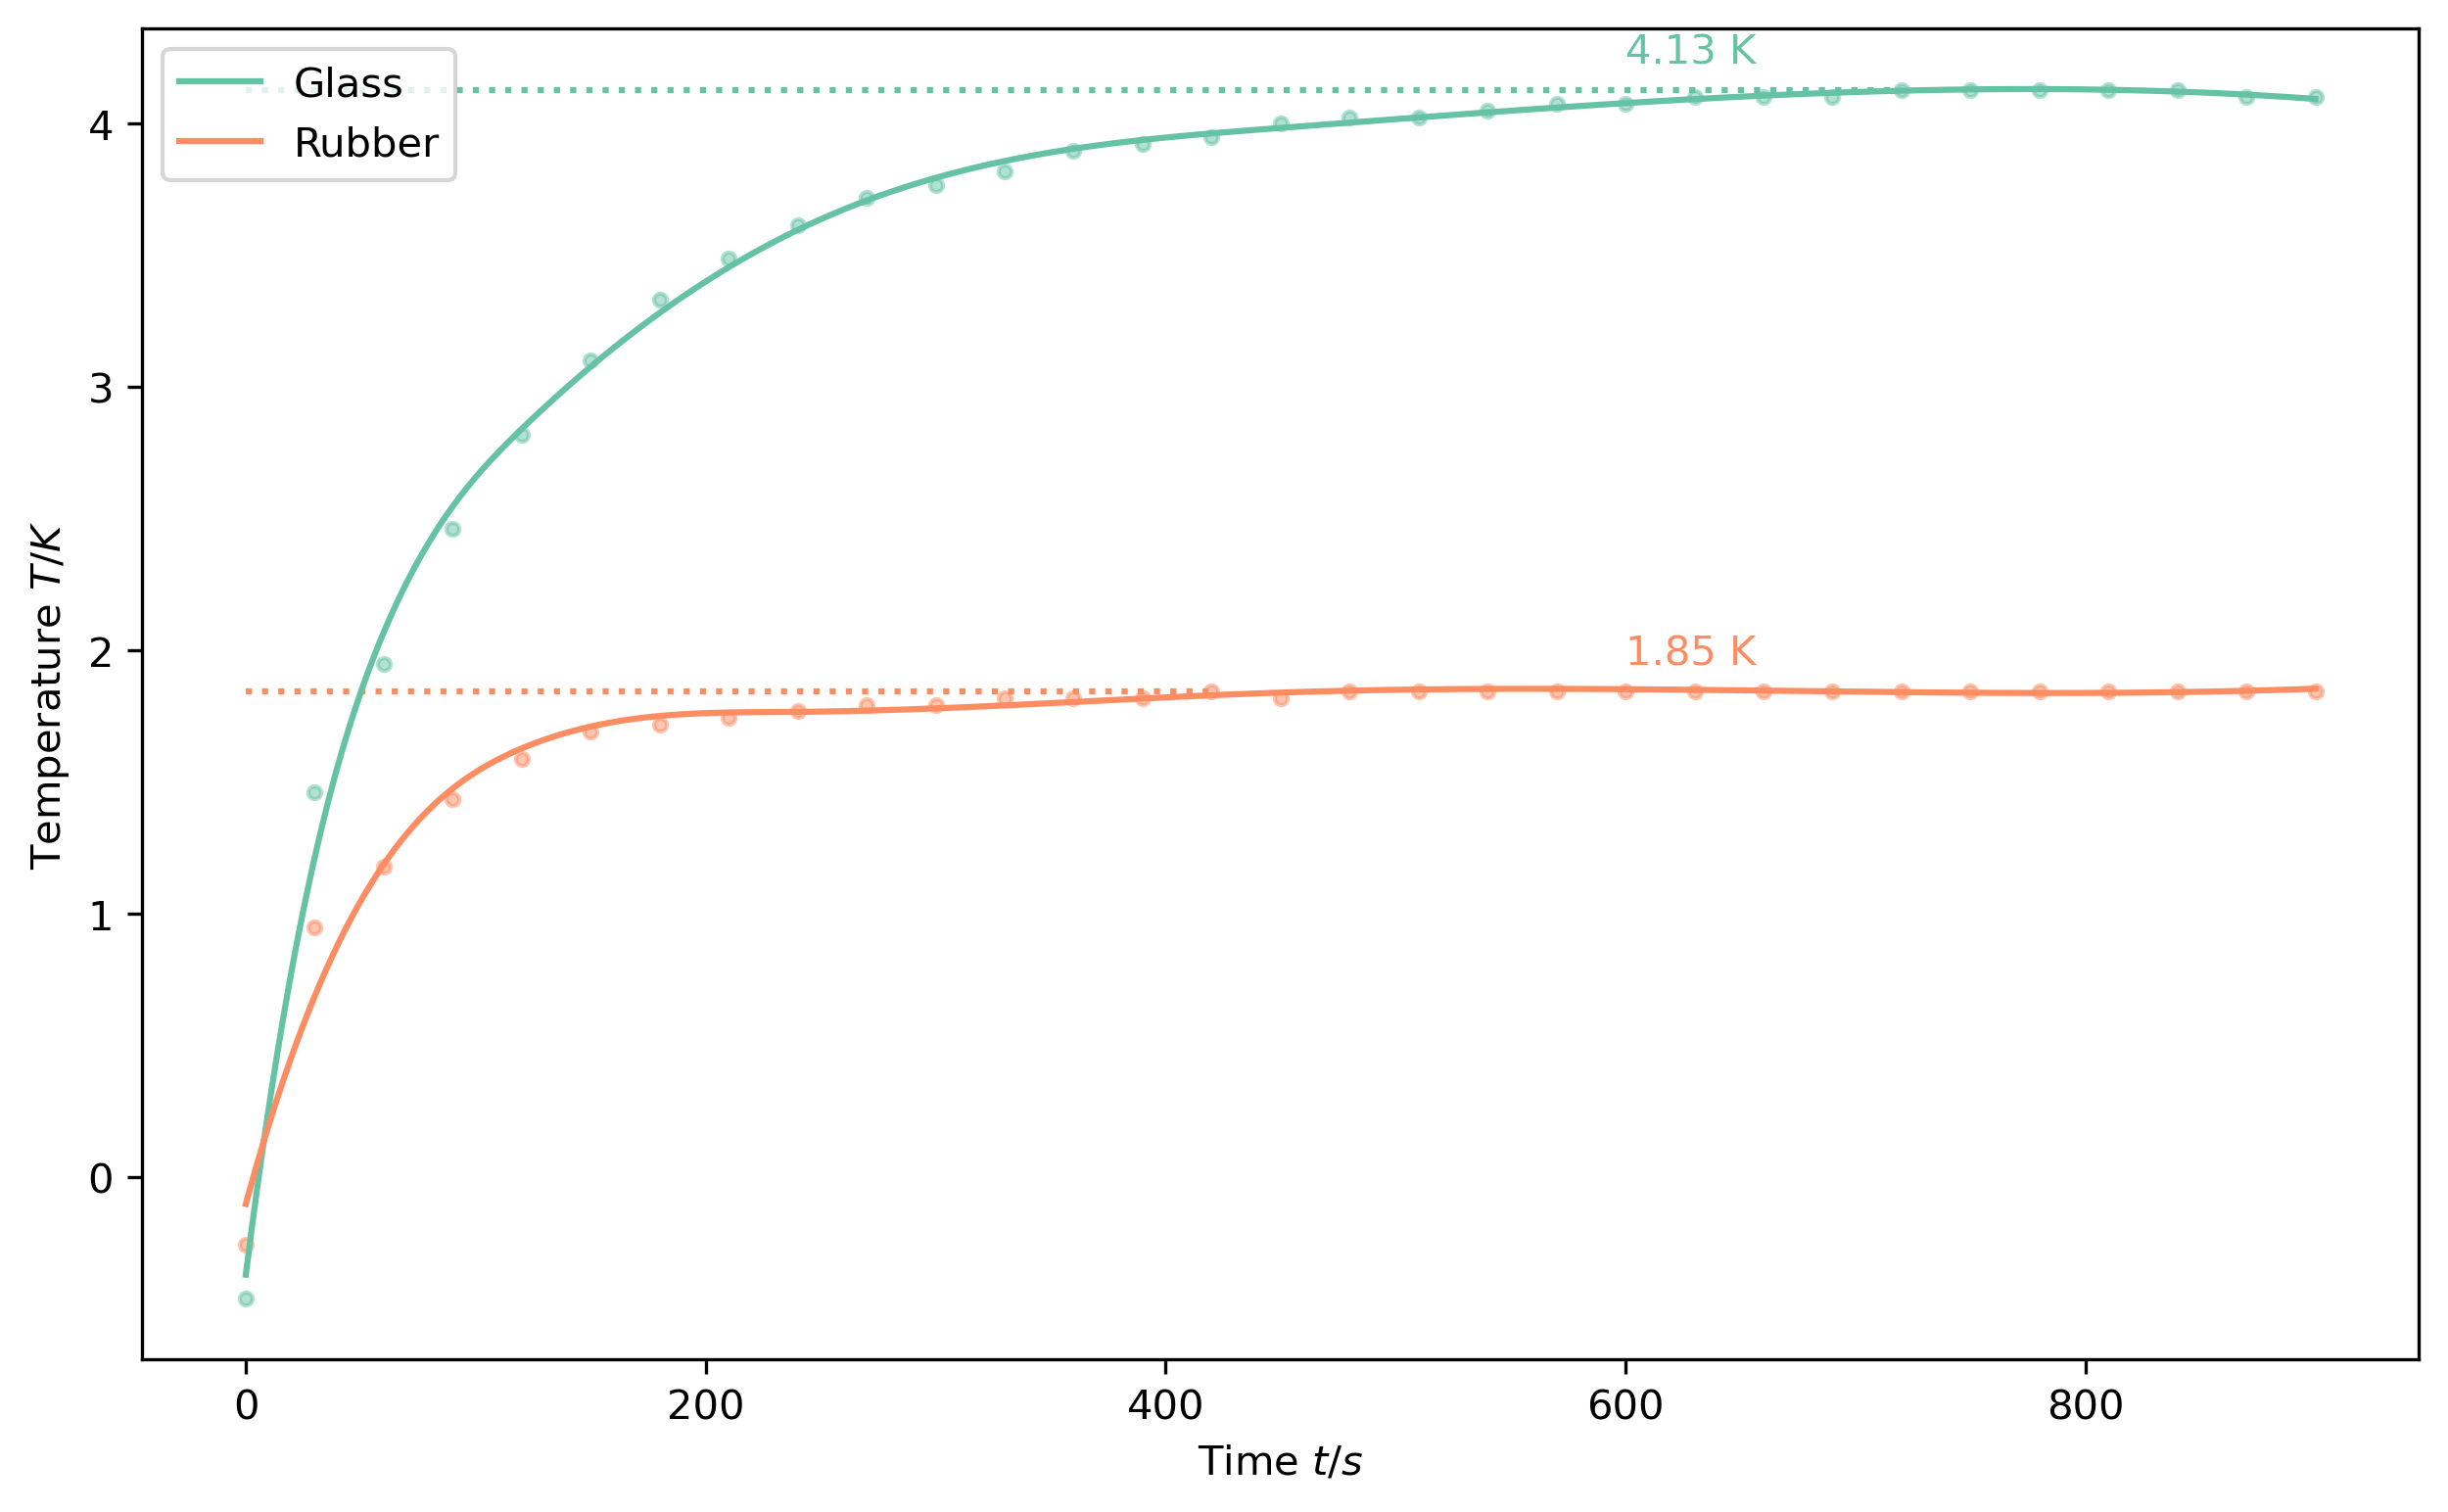
\includegraphics[width=0.23\textwidth]{attachments/fig.2.1.png}
    }	

    \subfloat[重新闭合]{
    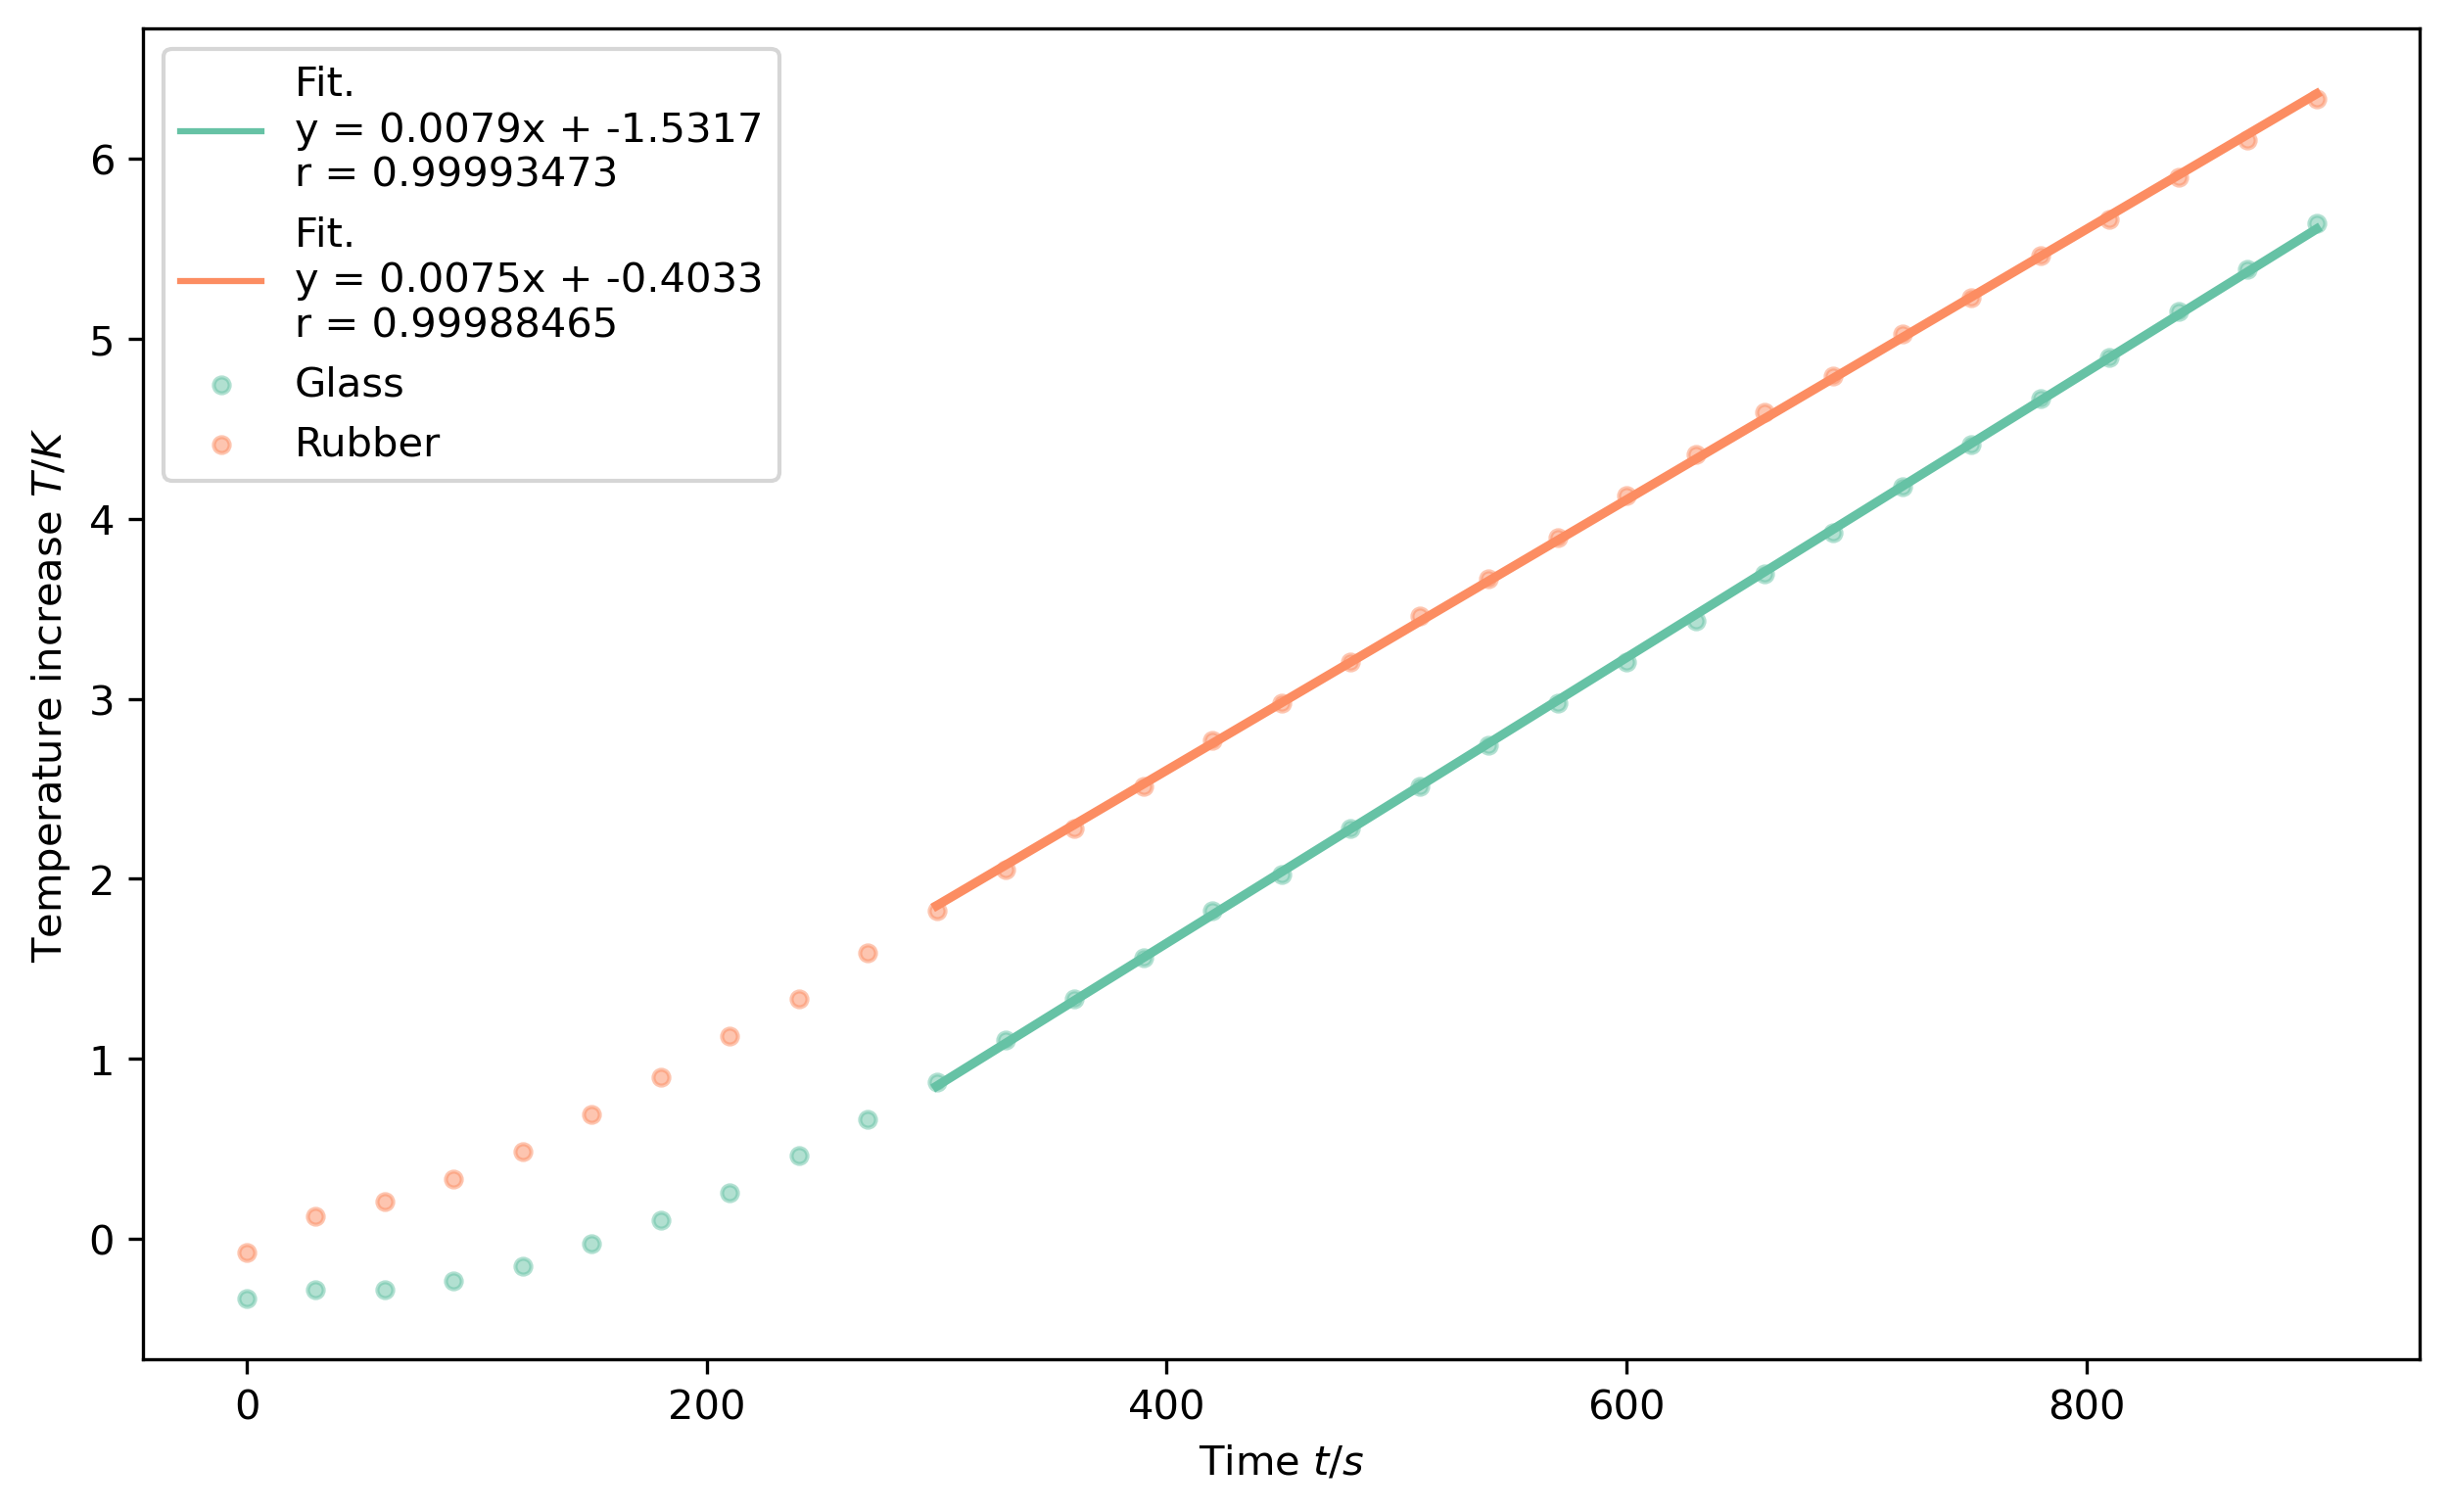
\includegraphics[width=0.23\textwidth]{attachments/fig.2.2.png}
    }
    \subfloat[第二次断开]{
    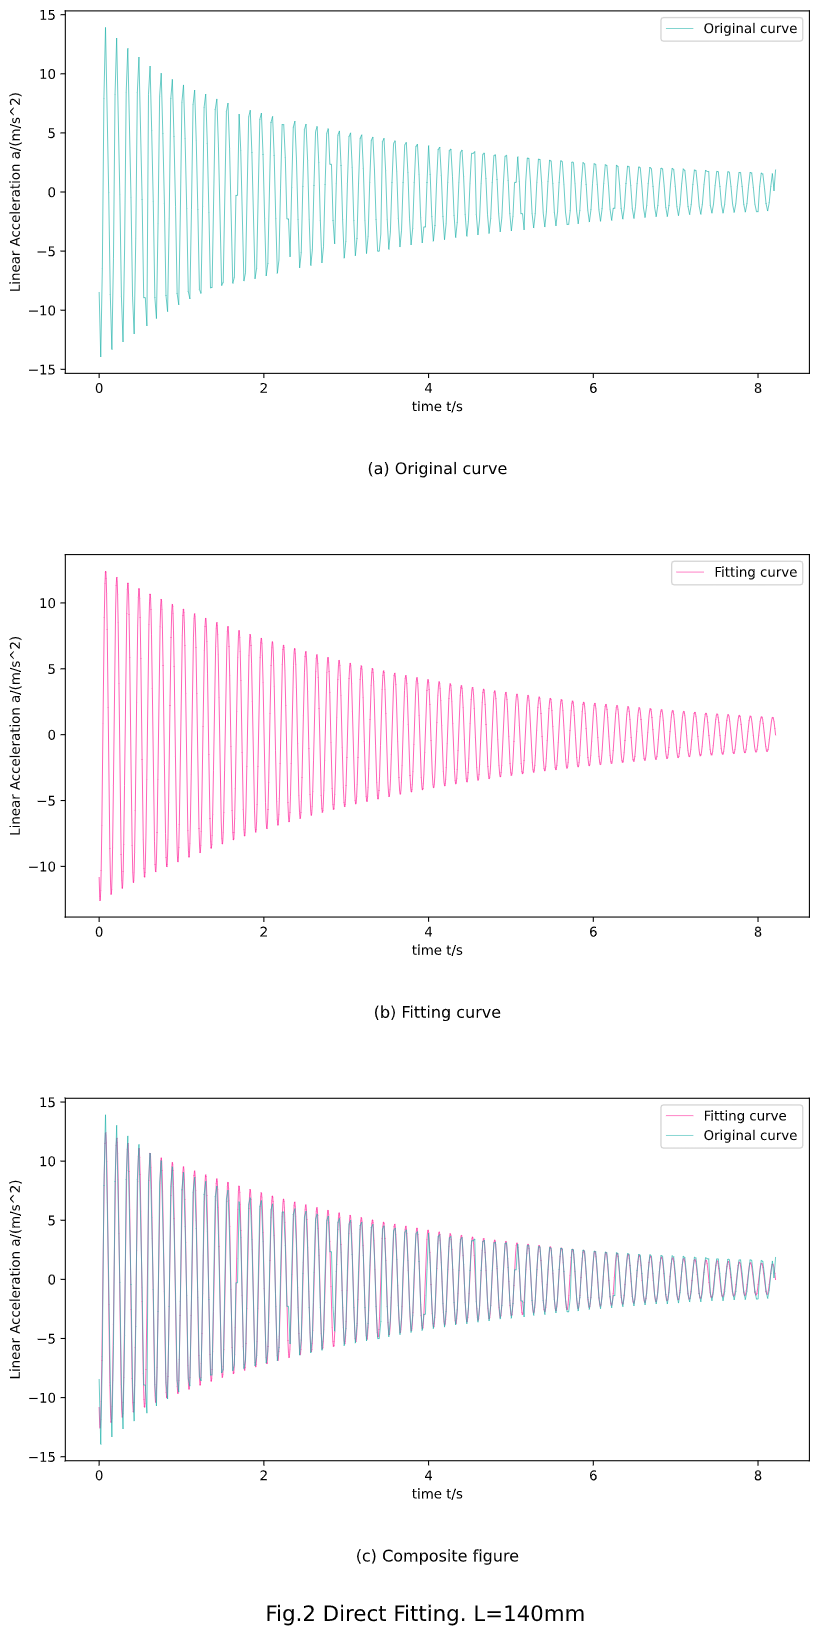
\includegraphics[width=0.23\textwidth]{attachments/fig.2.3.png}
    }	

    \subfloat[重新闭合]{
    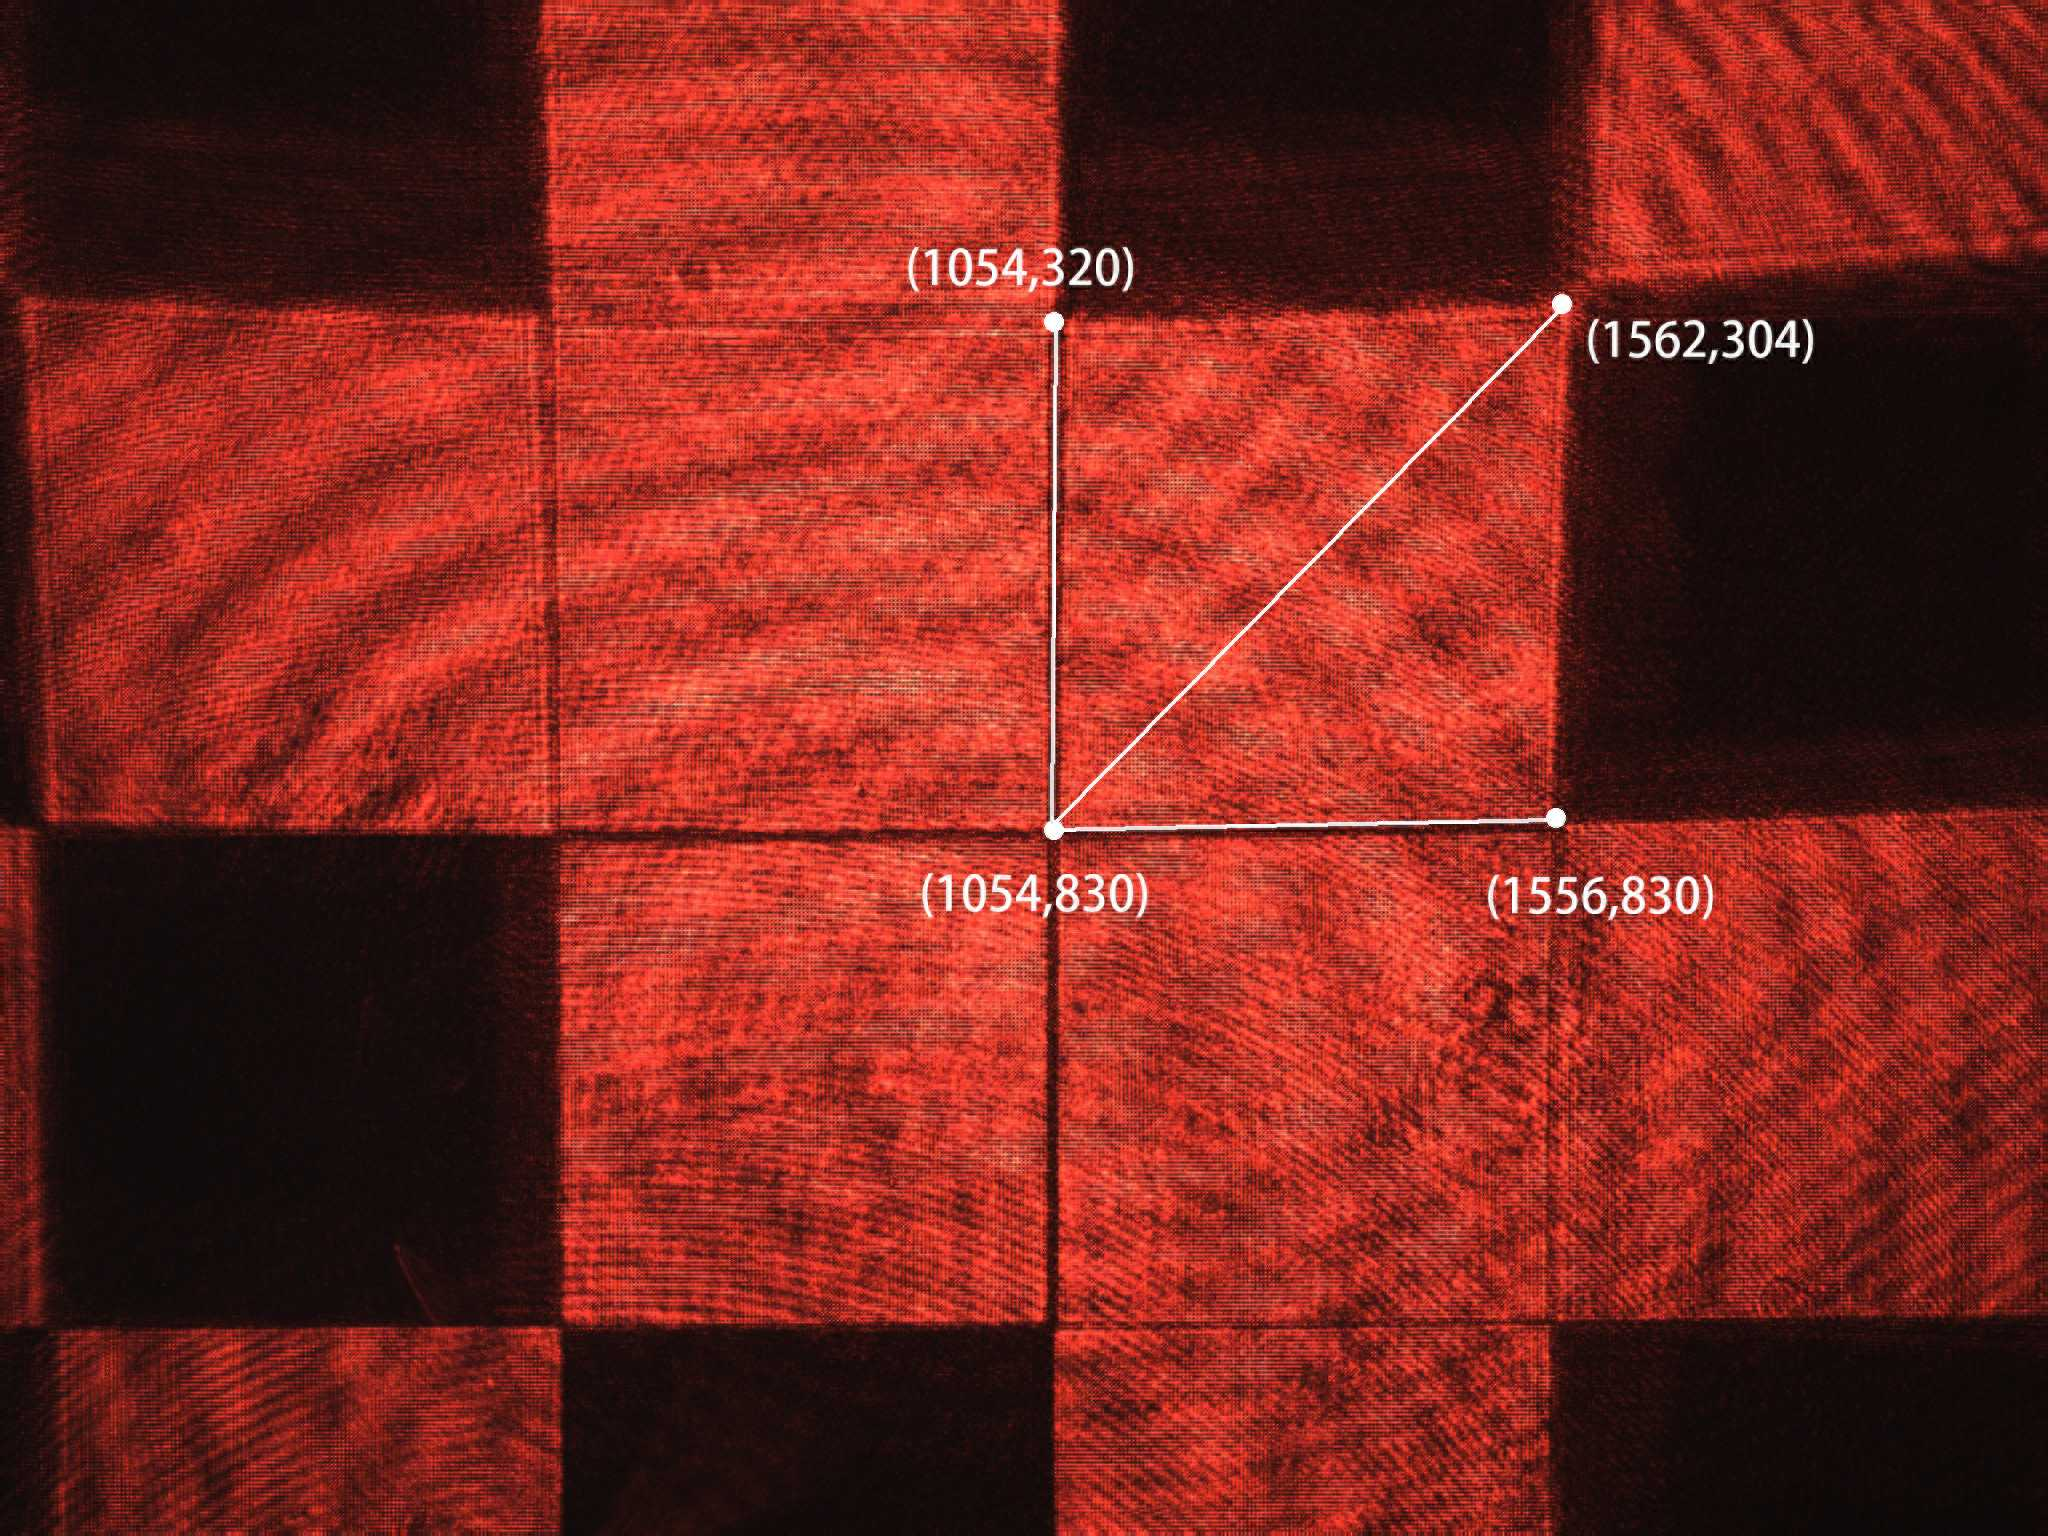
\includegraphics[width=0.23\textwidth]{attachments/fig.2.4.png}
    }
    \subfloat[第三次断开]{
    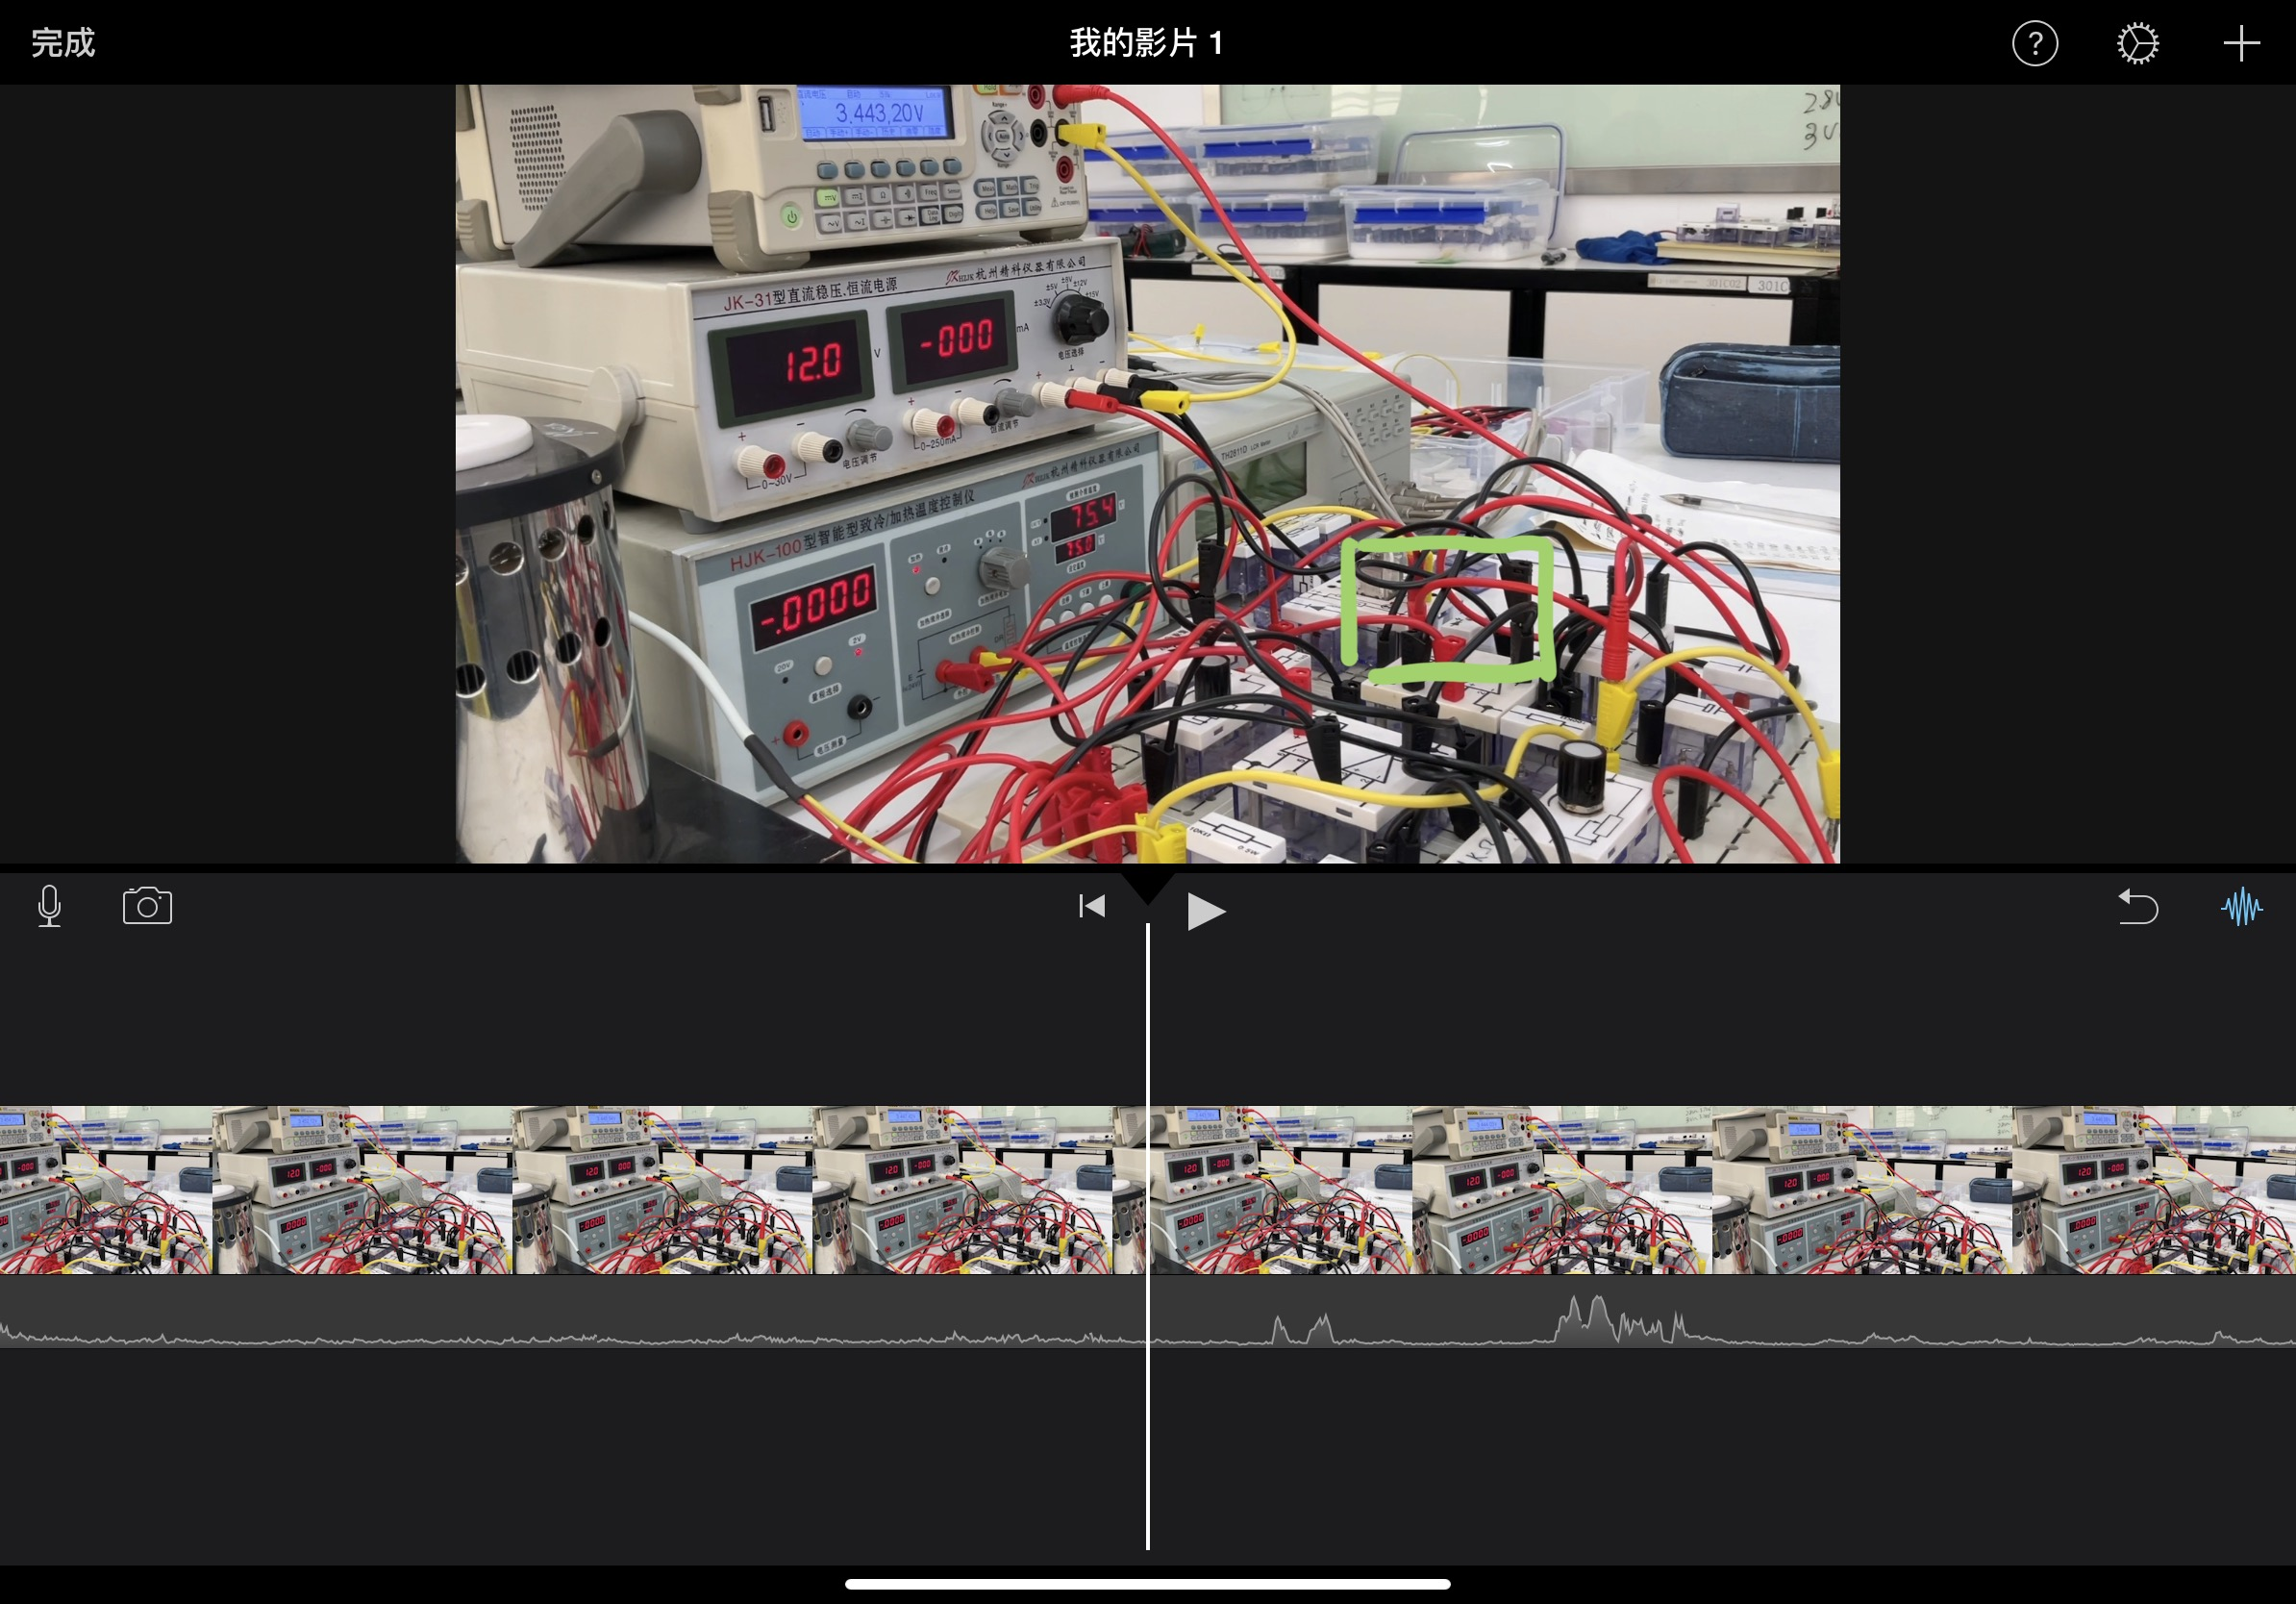
\includegraphics[width=0.23\textwidth]{attachments/fig.2.5.png}
    }	

    \subfloat[重新闭合]{
    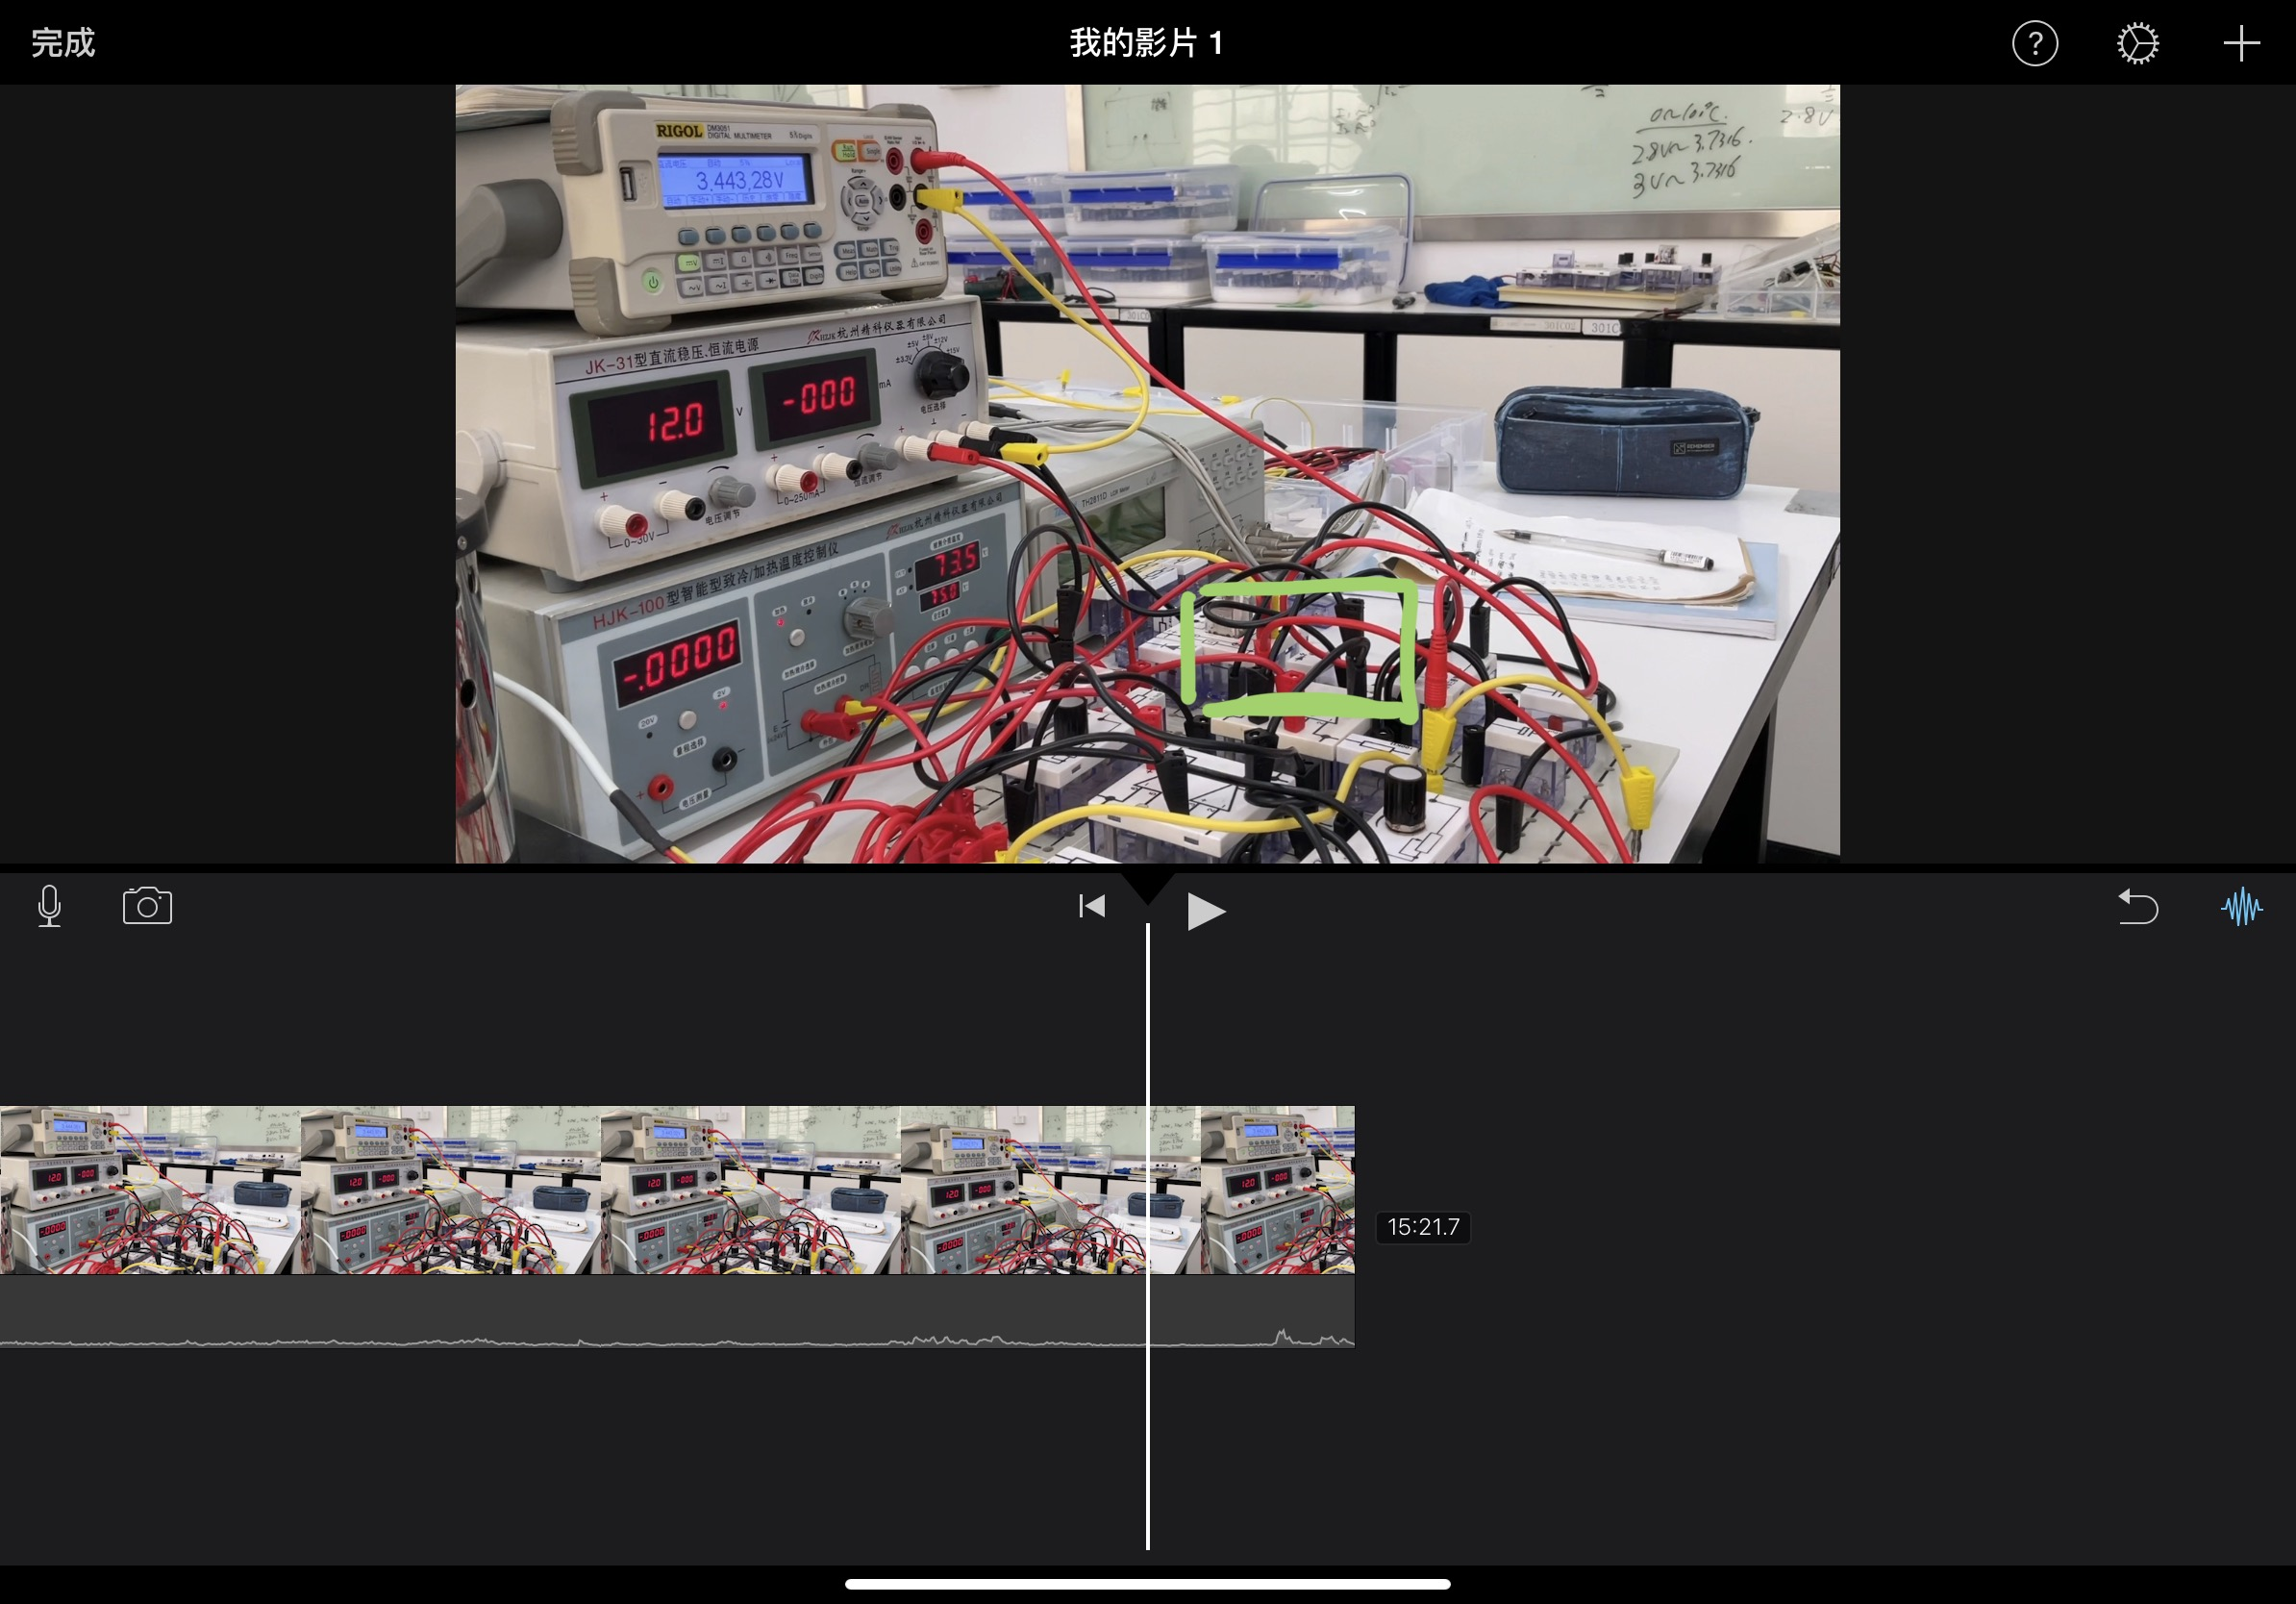
\includegraphics[width=0.23\textwidth]{attachments/fig.2.6.png}
    }
    \caption{继电器导通和断开瞬间}
    \label{fig:2}
\end{figure}
  
\subsection*{【项目源码】}
\url{https://github.com/Jeg-Vet/SYSU-PHY-EXP/tree/main/B12-Temperature_measuring_and_controlling_instrument}
		
\end{document}